% -*- Mode:TeX -*-

%% IMPORTANT: The official thesis specifications are available at:
%%            http://libraries.mit.edu/archives/thesis-specs/
%%
%%            Please verify your thesis' formatting and copyright
%%            assignment before submission.  If you notice any
%%            discrepancies between these templates and the 
%%            MIT Libraries' specs, please let us know
%%            by e-mailing thesis@mit.edu

%% The documentclass options along with the pagestyle can be used to generate
%% a technical report, a draft copy, or a regular thesis.  You may need to
%% re-specify the pagestyle after you \include  cover.tex.  For more
%% information, see the first few lines of mitthesis.cls. 

%\documentclass[12pt,vi,twoside]{mitthesis}
%%
%%  If you want your thesis copyright to you instead of MIT, use the
%%  ``vi'' option, as above.
%%
%\documentclass[12pt,twoside,leftblank]{mitthesis}
%%
%% If you want blank pages before new chapters to be labelled ``This
%% Page Intentionally Left Blank'', use the ``leftblank'' option, as
%% above. 

\documentclass[12pt,twoside]{mitthesis}
% My packages
\usepackage{amsmath}
\usepackage{titlesec}
\usepackage{graphicx}

% Template packages
\usepackage{lgrind}
%% These have been added at the request of the MIT Libraries, because
%% some PDF conversions mess up the ligatures.  -LB, 1/22/2014
\usepackage{cmap}
\usepackage[T1]{fontenc}
\pagestyle{plain} 

% My function definitions
\DeclareMathOperator{\arctantwo}{arctan2}
\DeclareMathOperator{\AHTD}{AHTD}
\DeclareMathOperator{\RHTD}{RHTD}
\DeclareMathOperator{\RMSE}{RMSE}

% Custom title format using package titlesec
\titleformat{\chapter}{\huge\bf}{\thechapter}{20pt}{\huge\bf}

% Graphics path for graphicx
\graphicspath{ {images/} }

\begin{document}

% -*-latex-*-
% 
% For questions, comments, concerns or complaints:
% thesis@mit.edu
% 
%
% $Log: cover.tex,v $
% Revision 1.8  2008/05/13 15:02:15  jdreed
% Degree month is June, not May.  Added note about prevdegrees.
% Arthur Smith's title updated
%
% Revision 1.7  2001/02/08 18:53:16  boojum
% changed some \newpages to \cleardoublepages
%
% Revision 1.6  1999/10/21 14:49:31  boojum
% changed comment referring to documentstyle
%
% Revision 1.5  1999/10/21 14:39:04  boojum
% *** empty log message ***
%
% Revision 1.4  1997/04/18  17:54:10  othomas
% added page numbers on abstract and cover, and made 1 abstract
% page the default rather than 2.  (anne hunter tells me this
% is the new institute standard.)
%
% Revision 1.4  1997/04/18  17:54:10  othomas
% added page numbers on abstract and cover, and made 1 abstract
% page the default rather than 2.  (anne hunter tells me this
% is the new institute standard.)
%
% Revision 1.3  93/05/17  17:06:29  starflt
% Added acknowledgements section (suggested by tompalka)
% 
% Revision 1.2  92/04/22  13:13:13  epeisach
% Fixes for 1991 course 6 requirements
% Phrase "and to grant others the right to do so" has been added to 
% permission clause
% Second copy of abstract is not counted as separate pages so numbering works
% out
% 
% Revision 1.1  92/04/22  13:08:20  epeisach

% NOTE:
% These templates make an effort to conform to the MIT Thesis specifications,
% however the specifications can change.  We recommend that you verify the
% layout of your title page with your thesis advisor and/or the MIT 
% Libraries before printing your final copy.
\title{A Thesis Title}

\author{Allison Schneider}
% If you wish to list your previous degrees on the cover page, use the 
% previous degrees command:
%       \prevdegrees{A.A., Harvard University (1985)}
% You can use the \\ command to list multiple previous degrees
%       \prevdegrees{B.S., University of California (1978) \\
%                    S.M., Massachusetts Institute of Technology (1981)}
\department{Dept. of Earth, Atmospheric and Planetary Sciences}

% If the thesis is for two degrees simultaneously, list them both
% separated by \and like this:
% \degree{Doctor of Philosophy \and Master of Science}
\degree{Bachelor of Science in Earth, Atmospheric and Planetary Sciences}

% As of the 2007-08 academic year, valid degree months are September, 
% February, or June.  The default is June.
\degreemonth{September}
\degreeyear{2017}
\thesisdate{August 5, 2017}

%% By default, the thesis will be copyrighted to MIT.  If you need to copyright
%% the thesis to yourself, just specify the `vi' documentclass option.  If for
%% some reason you want to exactly specify the copyright notice text, you can
%% use the \copyrightnoticetext command.  
%\copyrightnoticetext{\copyright IBM, 1990.  Do not open till Xmas.}

% If there is more than one supervisor, use the \supervisor command
% once for each.
\supervisor{Glenn R. Flierl}{Professor of Oceanography}

% This is the department committee chairman, not the thesis committee
% chairman.  You should replace this with your Department's Committee
% Chairman.
\chairman{???}{Chairman, Committee on Undergraduate Program}

% Make the titlepage based on the above information.  If you need
% something special and can't use the standard form, you can specify
% the exact text of the titlepage yourself.  Put it in a titlepage
% environment and leave blank lines where you want vertical space.
% The spaces will be adjusted to fill the entire page.  The dotted
% lines for the signatures are made with the \signature command.
\maketitle

% The abstractpage environment sets up everything on the page except
% the text itself.  The title and other header material are put at the
% top of the page, and the supervisors are listed at the bottom.  A
% new page is begun both before and after.  Of course, an abstract may
% be more than one page itself.  If you need more control over the
% format of the page, you can use the abstract environment, which puts
% the word "Abstract" at the beginning and single spaces its text.

%% You can either \input (*not* \include) your abstract file, or you can put
%% the text of the abstract directly between the \begin{abstractpage} and
%% \end{abstractpage} commands.

% First copy: start a new page, and save the page number.
\cleardoublepage
% Uncomment the next line if you do NOT want a page number on your
% abstract and acknowledgments pages.
% \pagestyle{empty}
\setcounter{savepage}{\thepage}
\begin{abstractpage}
% $Log: abstract.tex,v $
% Revision 1.1  93/05/14  14:56:25  starflt
% Initial revision
% 
% Revision 1.1  90/05/04  10:41:01  lwvanels
% Initial revision
% 
%
%% The text of your abstract and nothing else (other than comments) goes here.
%% It will be single-spaced and the rest of the text that is supposed to go on
%% the abstract page will be generated by the abstractpage environment.  This
%% file should be \input (not \include 'd) from cover.tex.
In this thesis, I designed and implemented a compiler which performs
optimizations that reduce the number of low-level floating point operations
necessary for a specific task; this involves the optimization of chains of
floating point operations as well as the implementation of a ``fixed'' point
data type that allows some floating point operations to simulated with integer
arithmetic.  The source language of the compiler is a subset of C, and the
destination language is assembly language for a micro-floating point CPU.  An
instruction-level simulator of the CPU was written to allow testing of the
code.  A series of test pieces of codes was compiled, both with and without
optimization, to determine how effective these optimizations were.

\end{abstractpage}

% Additional copy: start a new page, and reset the page number.  This way,
% the second copy of the abstract is not counted as separate pages.
% Uncomment the next 6 lines if you need two copies of the abstract
% page.
% \setcounter{page}{\thesavepage}
% \begin{abstractpage}
% % $Log: abstract.tex,v $
% Revision 1.1  93/05/14  14:56:25  starflt
% Initial revision
% 
% Revision 1.1  90/05/04  10:41:01  lwvanels
% Initial revision
% 
%
%% The text of your abstract and nothing else (other than comments) goes here.
%% It will be single-spaced and the rest of the text that is supposed to go on
%% the abstract page will be generated by the abstractpage environment.  This
%% file should be \input (not \include 'd) from cover.tex.
In this thesis, I designed and implemented a compiler which performs
optimizations that reduce the number of low-level floating point operations
necessary for a specific task; this involves the optimization of chains of
floating point operations as well as the implementation of a ``fixed'' point
data type that allows some floating point operations to simulated with integer
arithmetic.  The source language of the compiler is a subset of C, and the
destination language is assembly language for a micro-floating point CPU.  An
instruction-level simulator of the CPU was written to allow testing of the
code.  A series of test pieces of codes was compiled, both with and without
optimization, to determine how effective these optimizations were.

% \end{abstractpage}

\cleardoublepage

\section*{Acknowledgments}

This is the acknowledgements section.  You should replace this with your
own acknowledgements.

%%%%%%%%%%%%%%%%%%%%%%%%%%%%%%%%%%%%%%%%%%%%%%%%%%%%%%%%%%%%%%%%%%%%%%
% -*-latex-*-

% Some departments (e.g. 5) require an additional signature page.  See
% signature.tex for more information and uncomment the following line if
% applicable.
% % -*- Mode:TeX -*-
%
% Some departments (e.g. Chemistry) require an additional cover page
% with signatures of the thesis committee.  Please check with your
% thesis advisor or other appropriate person to determine if such a 
% page is required for your thesis.  
%
% If you choose not to use the "titlepage" environment, a \newpage
% commands, and several \vspace{\fill} commands may be necessary to
% achieve the required spacing.  The \signature command is defined in
% the "mitthesis" class
%
% The following sample appears courtesy of Ben Kaduk <kaduk@mit.edu> and
% was used in his June 2012 doctoral thesis in Chemistry. 

\begin{titlepage}
\begin{large}
This doctoral thesis has been examined by a Committee of the Department
of Chemistry as follows:

\signature{Professor Jianshu Cao}{Chairman, Thesis Committee \\
   Professor of Chemistry}

\signature{Professor Troy Van Voorhis}{Thesis Supervisor \\
   Associate Professor of Chemistry}

\signature{Professor Robert W. Field}{Member, Thesis Committee \\
   Haslam and Dewey Professor of Chemistry}
\end{large}
\end{titlepage}


\pagestyle{plain}
  % -*- Mode:TeX -*-
%% This file simply contains the commands that actually generate the table of
%% contents and lists of figures and tables.  You can omit any or all of
%% these files by simply taking out the appropriate command.  For more
%% information on these files, see appendix C.3.3 of the LaTeX manual. 
\tableofcontents
\newpage
\listoffigures
\newpage
\listoftables


%% This is an example first chapter.  You should put chapter/appendix that you
%% write into a separate file, and add a line \include{yourfilename} to
%% main.tex, where `yourfilename.tex' is the name of the chapter/appendix file.
%% You can process specific files by typing their names in at the 
%% \files=
%% prompt when you run the file main.tex through LaTeX.
\chapter{Introduction}

\section{The Aerocene Project}

\section{Geopotential Height}


%% To include in intro
% Geopotential height explanation
%% This is an example first chapter.  You should put chapter/appendix that you
%% write into a separate file, and add a line \include{yourfilename} to
%% main.tex, where `yourfilename.tex' is the name of the chapter/appendix file.
%% You can process specific files by typing their names in at the 
%% \files=
%% prompt when you run the file main.tex through LaTeX.
\chapter{Methods}

Two trajectory calculation routines, a kinematic and a dynamic model, were written using Python's NumPy scientific computing package.
Both routines numerically predict the trajectories of an ensemble of parcels by determining the velocities of parcels over time. 
The kinematic routine finds these velocities by interpolating between grids of wind speed data. 
The dynamic routine calculates velocities using advection equations relating the parcel acceleration and the geopotential height of a given pressure level. 

\section{Ten Day Dataset}
Data from the Global Forecast System (GFS), a weather forecast model produced by the National Centers for Environmental Protection (NCEP), was used for both models.
The dataset chosen was a ten day forecast, starting at 12:00:00 on February 21st, 2017, with predictions at intervals of three hours.
Each file in the dataset contains atmospheric predictions for the beginning of a three-hour interval. 
The values of atmospheric variables are predicted at each point on a latitude-longitude grid spanning the globe, with a spacing between gridpoints of 0.25 degree.
Values are predicted for East-West and North-South wind speed components $u$ and $v$, as well as the geopotential height $Z_g$ of the 250 millibar pressure level.

\section{Linear Interpolation}
Both the kinematic and dynamic models require an interpolation scheme to produce values for atmospheric variables at positions between the gridded values provided by GFS. 
Linear interpolation is the standard choice for trajectory models \cite{bowman_input_2013}. 
For both models, linear interpolation was used in three dimensions (latitude, longitude, and time). 
In the kinematic model, $u$ and $v$ components of wind speed were interpolated, while in the dynamic model, geopotential height was interpolated.

\section{Second-order Integration Scheme}
The numerical scheme chosen was a second-order Runge-Kutta method with a long track record in trajectory modeling \cite{petterssen_weather_1940}.
The velocity at a given timestep is taken to be the average of the velocity at the initial position and the velocity at the first-guess position after one timestep.

The first guess position $\vec{P}' (t + \Delta t)$ is 
\begin{align}
\vec{P}' (t + \Delta t) = \vec{P}(t) + \vec{V} (\vec{P}, t) \Delta t
\end{align}

and the final position $\vec{P} (t + \Delta t)$ is
\begin{align}
\vec{P} (t + \Delta t) = \vec{P} (t) + \frac{1}{2} \left [ \vec{V} (\vec{P}, t) + \vec{V} (\vec{P'}, t + \Delta t) \right ] \Delta t
\end{align}

where $\vec{P}$ is a position vector with latitude and longitude components, and $\vec{V}$ a velocity vector with $u$ and $v$ wind speeds \cite{draxler_description_1997}.
This integration method is used by HYSPLIT and a number of other trajectory models, including FLEXPART, LAGRANTO, and STILT \cite{stein_noaas_2015} \cite{bowman_input_2013}. 
For trajectories calculated from interpolated gridded wind velocities, higher order integration schemes do not add precision \cite{draxler_description_1997}.  

\section{Constant Timestep}
The timestep for integration was three minutes, with the timestep throughout the trajectory. 
To save computation, HYSPLIT uses a dynamic timestep, varying from one minute to one hour, computed to satisfy

\begin{align}
U_{max} [\text{grid-units min}^{-1}] \Delta t [\text{min}] < 0.75 [\text{grid-units}] 
\end{align}

\cite{draxler_description_1997}. This ensures that the parcel does not blow past any grid squares during a single timestep, which maximizes the accuracy of the calculation. 
[Todo: Plot u and v along my trajectories to see if the $U_{max} \Delta t < 0.75$ relation is always satisfied. If it isn't, consider reducing the timestep. If it is satisfied, write that here.]

\section{Kinematic Equations}
At each timestep, after $u$ and $v$ speeds were interpolated and an average value found using the integration scheme, the kinematic model used two equations to solve for a parcel's displacement. 
Since GFS provides $u$ and $v$ values in meters per second, the equations convert from Cartesian to geographic coordinates. 
The $r$ value of a parcel is taken to be the radius of the Earth $R_E$ plus the parcel's geopotential height $Z_g$.

\begin{align}
r &= R_E + Z_g \\[2ex]
\frac{d \varphi}{dt} &= \frac{v}{r} \\
\frac{d \lambda}{dt} &= \frac{u}{r \cos{\varphi}}
\end{align}

\section{Dynamic Equations}
In the dynamic model, velocity at the next timestep was calculated using advection equations which incorporate the current geopotential height gradient and the previous timestep's $u$ and $v$ values.
The Coriolis parameter $f$ measures the effect of the Earth's rotation speed $\Omega$ at a given latitude $\varphi$.
Standard acceleration due to gravity is $g$. 

\begin{align}
f &= 2 \Omega \sin{\varphi} \\[2ex]
\frac{du}{dt} &= g \frac{\partial Z_g}{\partial \lambda} + fv \\
\frac{dv}{dt} &= g \frac{\partial Z_g}{\partial \varphi} - fu
\end{align}

\section{Mean Trajectory and RMSE}
For an ensemble of parcels, variance among trajectories over time was measured by calculating the mean trajectory: the path of an imaginary parcel whose position at each timestep is the average of the parcels' positions.
At each timestep, the root-mean-square error (RMSE) is the square root of the average squared value of each particle's distance from the mean trajectory.

The mean trajectory was determined by finding the centroids of parcel positions at each timestep after converting trajectory latitudes and longitudes to Cartesian coordinates. 
NumPy's \texttt{arctan2(y,x)} is a two-argument arctangent function with a range of $(-\pi, \pi]$.

\begin{align}
x &= \cos \varphi \cos \lambda & \bar{x} &= \frac{x_1 + x_2 + \cdots + x_n}{n} \\
y &= \cos \varphi \sin \lambda & \bar{y} &= \frac{y_1 + y_2 + \cdots + y_n}{n} \\
z &= \sin \varphi & \bar{z} &= \frac{z_1 + z_2 + \cdots + z_n}{n} \\[2ex]
\bar{\lambda} &= \arctantwo{(\bar{y},\bar{x})} \\
\bar{\varphi} &= \arctantwo{(\bar{z}, \sqrt{\bar{x}^2 + \bar{y}^2})}
\end{align}

The distance $d$ between each parcel (with position $\varphi_i, \lambda_i$) and the mean parcel was calculated with the haversine formula

\begin{align}
\Delta \varphi_i &= | \varphi_i - \bar{\varphi}| \\
\Delta \lambda_i &= |\lambda_i - \bar{\lambda}| \\
a_i &= \sin^2 \left ( \frac{\Delta \varphi}{2} \right ) + \cos{\varphi_1}  \cos{\varphi_2} \sin^2 \left ( \frac{\Delta \lambda}{2} \right ) \\
c_i &= 2 \cdot \arctantwo{(\sqrt{a}, \sqrt{1 - a})} \\
d_i &= R_E \cdot c
\end{align}

which is accurate and well-conditioned for small angles \cite{sinnott_virtues_1984}. 
The RMSE at each timestep is calculated using the distance between each parcel and the mean parcel.

\begin{align}
\text{RMSE} = \sqrt{\frac{{d_1}^2 + {d_2}^2 + \cdots + {d_n}^2}{n}}
\end{align}

\chapter{Tuning the Models}

\section{Inertial Circles in the Dynamic Model}

\begin{figure}
    
\includegraphics[width=0.5\textwidth]{force_180.eps}
    \centering
    \caption{Twenty five dynamic trajectories launched in an evenly-spaced grid with its lower-left corner at 41, -72 and upper-right corner at 42, -71. 
    The large spirals are implausible for jet stream flow and reflect a problem with the model.}
    \label{fig:force_180}
\end{figure}

\section{Adding Friction to the Dynamic Model}

[[[Inertial circles have been encountered before in dynamic models and there are different ways of dealing with them.]]] \cite{stohl_accuracy_1998}
One approach, used by Stohl and Seibert, is to take a weighted average of the wind speeds from the dynamic model and interpolated speeds from a kinematic model at each timestep.
Another approach is to change the frictionless assumption of the dynamical model.
[[[Why does the force of friction damp oscillations?]]]
Using the definition of geostrophic wind in Equations \ref{eq:u_g} and \ref{eq:v_g}, Equations \ref{eq:uvelocitygeo} and \ref{eq:vvelocitygeo} with an added friction term become

\begin{align}
    \frac{du}{dt} &= f (v - v_g) - r_f (u - u_g) \\
    \frac{dv}{dt} &= -f (u - u_g) - r_f (v - v_g).   
\end{align}

The friction parameter $r_f$ is analogous to the Coriolis parameter: it has units of second$^{-1}$ and is a measure of the force of friction.

\section{Choosing a Timestep} \label{sec:timestep}
test

\begin{figure}
    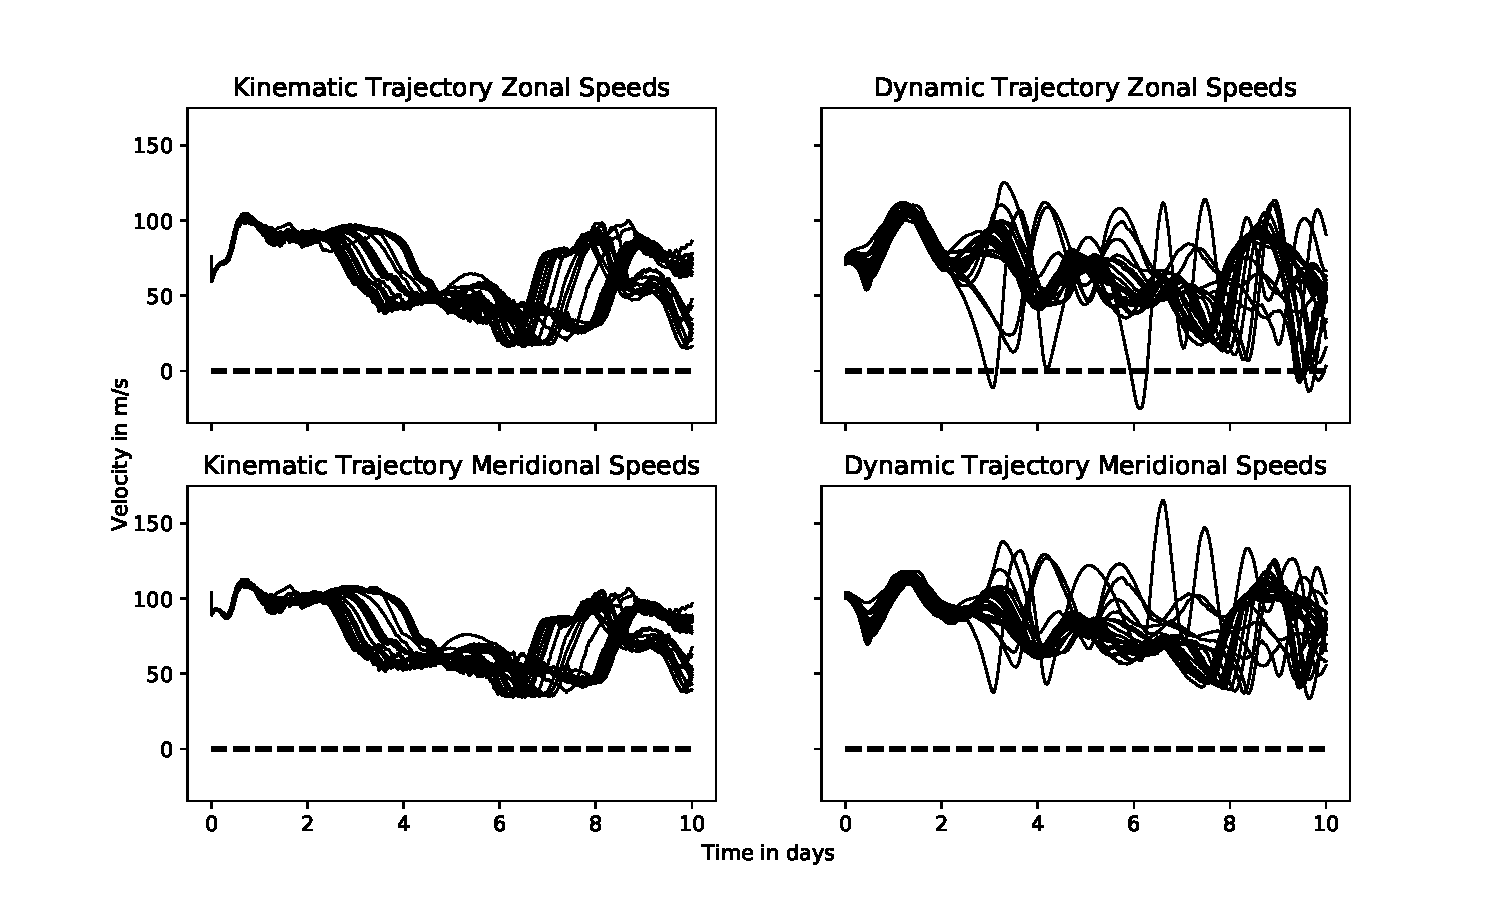
\includegraphics[width=\textwidth]{speed_subplots_180.pdf}
    \centering
    \caption{For a timestep of 3 minutes, [[[blah blah]]]}
    \label{}
\end{figure}

\begin{figure}
    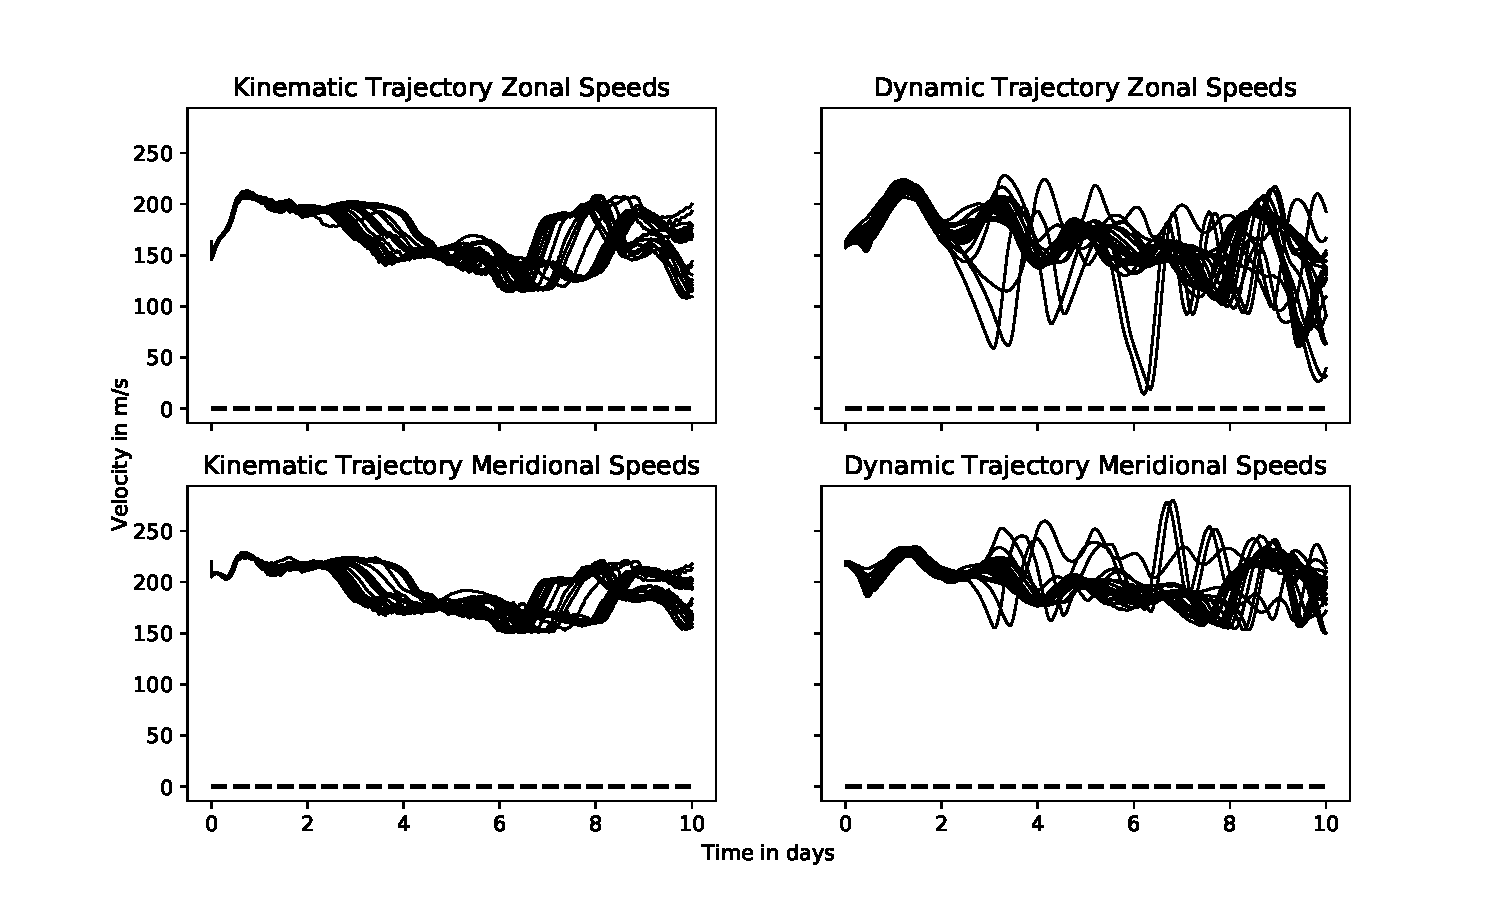
\includegraphics[width=\textwidth]{speed_subplots_90.pdf}
    \centering
    \caption{For a timestep of 1 minute 30 seconds, [[[blah blah]]]}
    \label{}
\end{figure}

%% This defines the bibliography file (main.bib) and the bibliography style.
%% If you want to create a bibliography file by hand, change the contents of
%% this file to a `thebibliography' environment.  For more information 
%% see section 4.3 of the LaTeX manual.
\begin{singlespace}
\bibliography{main}
\bibliographystyle{apalike}
\end{singlespace}

\end{document}

